\documentclass{article}
\usepackage[top=1in, bottom=1in, left=1in, right=1in]{geometry}
% \usepackage{fullpage, fancyhdr}
\usepackage{fullpage}
\usepackage{float}
\usepackage{mathtools}
\usepackage{xfrac}
\usepackage{graphicx}
\usepackage{caption}
\usepackage{subcaption}
\usepackage{portland}
%\usepackage{setspace}
\setlength{\topmargin}{0.0in}
\setlength{\headheight}{0.5in}
\setlength{\headsep}{0in}
\setlength{\footskip}{9pt}
\usepackage{listings}
\usepackage{color}

\usepackage{multicol}

\renewcommand{\arraystretch}{1.5}

% For circuitikz
\usepackage[american,arrowmos]{circuitikz}
\usepackage{tikz}
\usetikzlibrary{calc}
\usepackage{pgfplots}
\usepackage{amsfonts}
\usetikzlibrary{shapes,arrows}

% \pagestyle{fancyplain}
\pagestyle{myheadings}
\voffset=-0.50in
\topmargin=0.00in 
\headsep=0.25in 
\evensidemargin=0in 
\oddsidemargin=0in 
\textwidth=6.6in 
\textheight=10.0in 

\renewcommand{\topfraction}{0.9}	% max fraction of floats at top
\renewcommand{\bottomfraction}{0.8}	% max fraction of floats at bottom
%   Parameters for TEXT pages (not float pages):
\setcounter{topnumber}{2}
\setcounter{bottomnumber}{2}
\setcounter{totalnumber}{4}     % 2 may work better
\setcounter{dbltopnumber}{2}    % for 2-column pages
\renewcommand{\dbltopfraction}{0.9}	% fit big float above 2-col. text
\renewcommand{\textfraction}{0.07}	% allow minimal text w. figs
%   Parameters for FLOAT pages (not text pages):
\renewcommand{\floatpagefraction}{0.7}	% require fuller float pages
% N.B.: floatpagefraction MUST be less than topfraction !!
\renewcommand{\dblfloatpagefraction}{0.7}	% require fuller float pages
% remember to use [htp] or [htpb] for placement

\title{Assignment \# 7: MEMS Pressure and Resistor Calculations}
\date{4/03/2013}
\author{Brian Arnberg}

\markright{Brian Arnberg\hfill ELEC 6760 - Solid State Sensors\hfill}     
\setlength{\parindent}{0pt}


\begin{document}\label{start}

% \begin{titlepage}
% 	\maketitle
% 	\thispagestyle{empty}
% \end{titlepage}


\section*{ Homework Assignment \#7 - Due Wed. 4/03/13 }
\renewcommand{\labelenumi}{\arabic{enumi})}
\begin{multicols}{2}
\begin{enumerate}
%--------------------------------------------------------------%
%---- Problem 1 -----------------------------------------------%
\item\label{p1}
 Estimate the depth in the ocean that the static pressure is 50\% due to the water
     depth and 50\% due to the air pressure above the water. Use 1G = 9.8 $m/s^2$ and 1
     $g/cm^3$ for the density of sea water, and 1atm for the air pressure.

		\begin{tabular}{ l }
			$P_t = P_w + P_{air} \colon P_w = P_{air}$\\
			$P_{air} = 1atm = 101.325kPa \colon P_w = \rho g h$\\
			$\rho g h = 1atm \rightarrow h = \frac{1atm}{\rho g}$\\
			$h = \frac{101.325kPa}{1000 kg/m^3 9.8m/s^2} = 10.3m$\\
			$\text{depth in the ocean} = 10.3 m$
		\end{tabular}
%--------------------------------------------------------------%
%---- Problem 2 -----------------------------------------------%
\item\label{p2}
A MEMS submarine is being used to monitor the cooling fluid in an industrial
     transformer. The transformer fluid (liquid) has a density of 2 $g/cm^3$. The sub is in
     motion and measures the total pressure (1960.1 Pa) and the static pressure (1960
     Pa) that it experiences, using gage pressure sensors. For 1G = 9.8 $m/s^2$, estimate
     the velocity of the sub in $mm/s$?

		\begin{tabular}{ l }
			$ \rho = 2 g/cm^3 = 2000kg/m^3$\\
			$P_t = 1960.1 Pa \colon P_s = 1960 Pa$\\
			$P_t = P_s + \frac{\rho v^2}{2} \rightarrow v=\sqrt{\frac{2(P_t - P_s)}{\rho}}$\\
			$v = \sqrt{\frac{2(1960.1 - 1960)}{2000}} = 100\mu m/s$\\
			$v = 0.100 mm/s$
		\end{tabular}
  
%--------------------------------------------------------------%
%---- Problem 3 -----------------------------------------------%
\item\label{p3}
For the sub in (\ref{p2}), what is the depth of the sub in mm, ignoring atmospheric
     pressure?

		\begin{tabular}{ l }
			$P_s = 1960 Pa \colon P_s = \rho g h$\\
			$1960 = (2000)(9.8)(h)\rightarrow h = 0.1m = 100mm$\\
			$\text{depth of the sub} = 100 mm$
		\end{tabular}
%--------------------------------------------------------------%
%---- Problem 4 -----------------------------------------------%
\item\label{p4}
For the pressure sensor diaphragm shown below, the four identical P-type
     piezoresistors have a gauge factor of +180:
     \begin{enumerate}
	\item Under pressure, is each resistor in compression or tension?

	\item Under pressure, has each resistor increased or decreased in resistance?
     \end{enumerate}

		\begin{tabular}{ l | c | c }
			Resistor & (a) & (b) \\ \hline
			$R_1$ & Tension & Increased\\
			$R_2$ & Compression & Decreased\\
			$R_3$ & Compression & Decreased\\
			$R_4$ & Tension & Increased\\
		\end{tabular}
  
%--------------------------------------------------------------%
%---- Problem 5 -----------------------------------------------%
\item\label{p5}
 Estimate the acceleration level of a shock event of a $1 Kg$ object falling $10m$ onto
     a hard surface where it completely stops moving 10$ms$ after initial impact. (1G =
     9.8 $m/s^2$)

		\begin{tabular}{ l }
			$V_0 = 0m/s \colon V_1 = g t_1$\\
			$d = 0.5 g {t_1}^2 \rightarrow t_1 = 1.428s$\\
			$V_1 = 9.8m/s^2 \times 1.428 s = 14m/s$\\
			$V_2 = 0m/s \colon t_2 = 10ms = 0.01s$\\
			$V_2 = a t_2 + V_1 \rightarrow a = \frac{V_2 - V_1}{t_2}$\\
			$a = \frac{-14m/s}{0.01s} = -1400m/s^2$\\
			$\text{shock acceleration} = 1400m/s^2 \approx 142.8\text{G's}$
		\end{tabular}

\end{enumerate}
\end{multicols}

\begin{figure}[h]
	\centering
	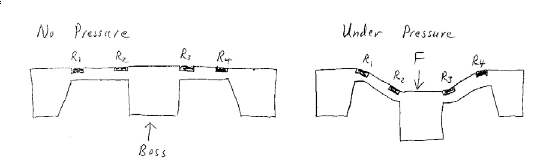
\includegraphics[keepaspectratio,width=\textwidth]{diaphragm}
\end{figure}

\label{end}\end{document}


